\documentclass[10pt]{scrartcl}
\usepackage{amsmath,amsthm,amssymb,mathtools,xfrac}
\usepackage{enumerate}
\usepackage[utf8]{inputenc}
%\usepackage{german}
\usepackage{a4wide}
\usepackage{graphics}
\usepackage{graphicx}
\usepackage[T1]{fontenc}
\usepackage{epsfig}
\usepackage{libertine}
\usepackage[pdftex]{hyperref}
\usepackage{refcount}
\usepackage{framed} 
\usepackage{xcolor}
\usepackage{multicol}
\usepackage{enumitem}
\usepackage{caption}
\usepackage{gensymb}
\usepackage[export]{adjustbox}

\topmargin-.5in \textheight9in \oddsidemargin0in \textwidth6.5in

\begin{document}


\begin{minipage}{.5\textwidth}
{\scshape Department of Mathematics and Informatics \\
University of Cologne\\}
\small Prof. Dr. Gregor Gassner \\
\small Dr. Andrés Rueda-Ramírez \\
\end{minipage}
\hfill
\begin{minipage}{.3\textwidth}
\begin{flushright}

\includegraphics[width=3cm]{figs/logo-uni-koeln.jpg}\\
\today
\end{flushright}
\end{minipage}

\begin{center}
{\Large\bfseries
An Introduction to Climate Modeling}\\
\vspace{0.2cm}
{\bfseries Milestone 6 - Fixing Stability in the spatial 2D Energy Balance Modell}
\end{center}



\section{Fixing Stability in the spatial 2D Energy Balance Model}
\begin{enumerate}

\item In the previous milestone you have implemented the spatial operator of the diffusive EBM for two spatial dimensions. The investigations of the eigenvalues revealed that the stable time step of the explicit Euler method is prohibitively small. Hence, we focus on the implicit Euler method. Adapt the function\\ 
csmall\texttt{\detokenize{calc_equilibrium_2d }}\normalsize to use the backward Euler instead of the forward Euler time integration method. Visualize the results as an animation.

\item  Use the functions \small\texttt{\detokenize{calc_area_mean}}\normalsize, \small\texttt{\detokenize{calc_area_mean_north }}\normalsize and \small\texttt{\detokenize{calc_area_mean_south }}\normalsize  from previous milestones to compute the mean temperature values from the EBM in two space dimensions. Compare them with the results in milestone 4. Compare also the results for the temperature in Cologne. What is noticeable?

\item  Write a function to compute equilibrium simulations based on NASA $CO_2$ data from 1980 to the present. Plot the results.

\item Now we want to investigate the sensitivity of the model to the parameters. Repeat the calculations of the temperature for the year 1950 with the parameters from Ziegler and Rehfeld 2021 \footnote{E. Ziegler and K.Rehfeld, {\em TransEBM v. 1.0: description, tuning, and validation of a transient model of the Earth's energy balance in two dimensions}, Geoscientific Model Development 14.5, 2021.}.:\\
\begin{figure}[h]
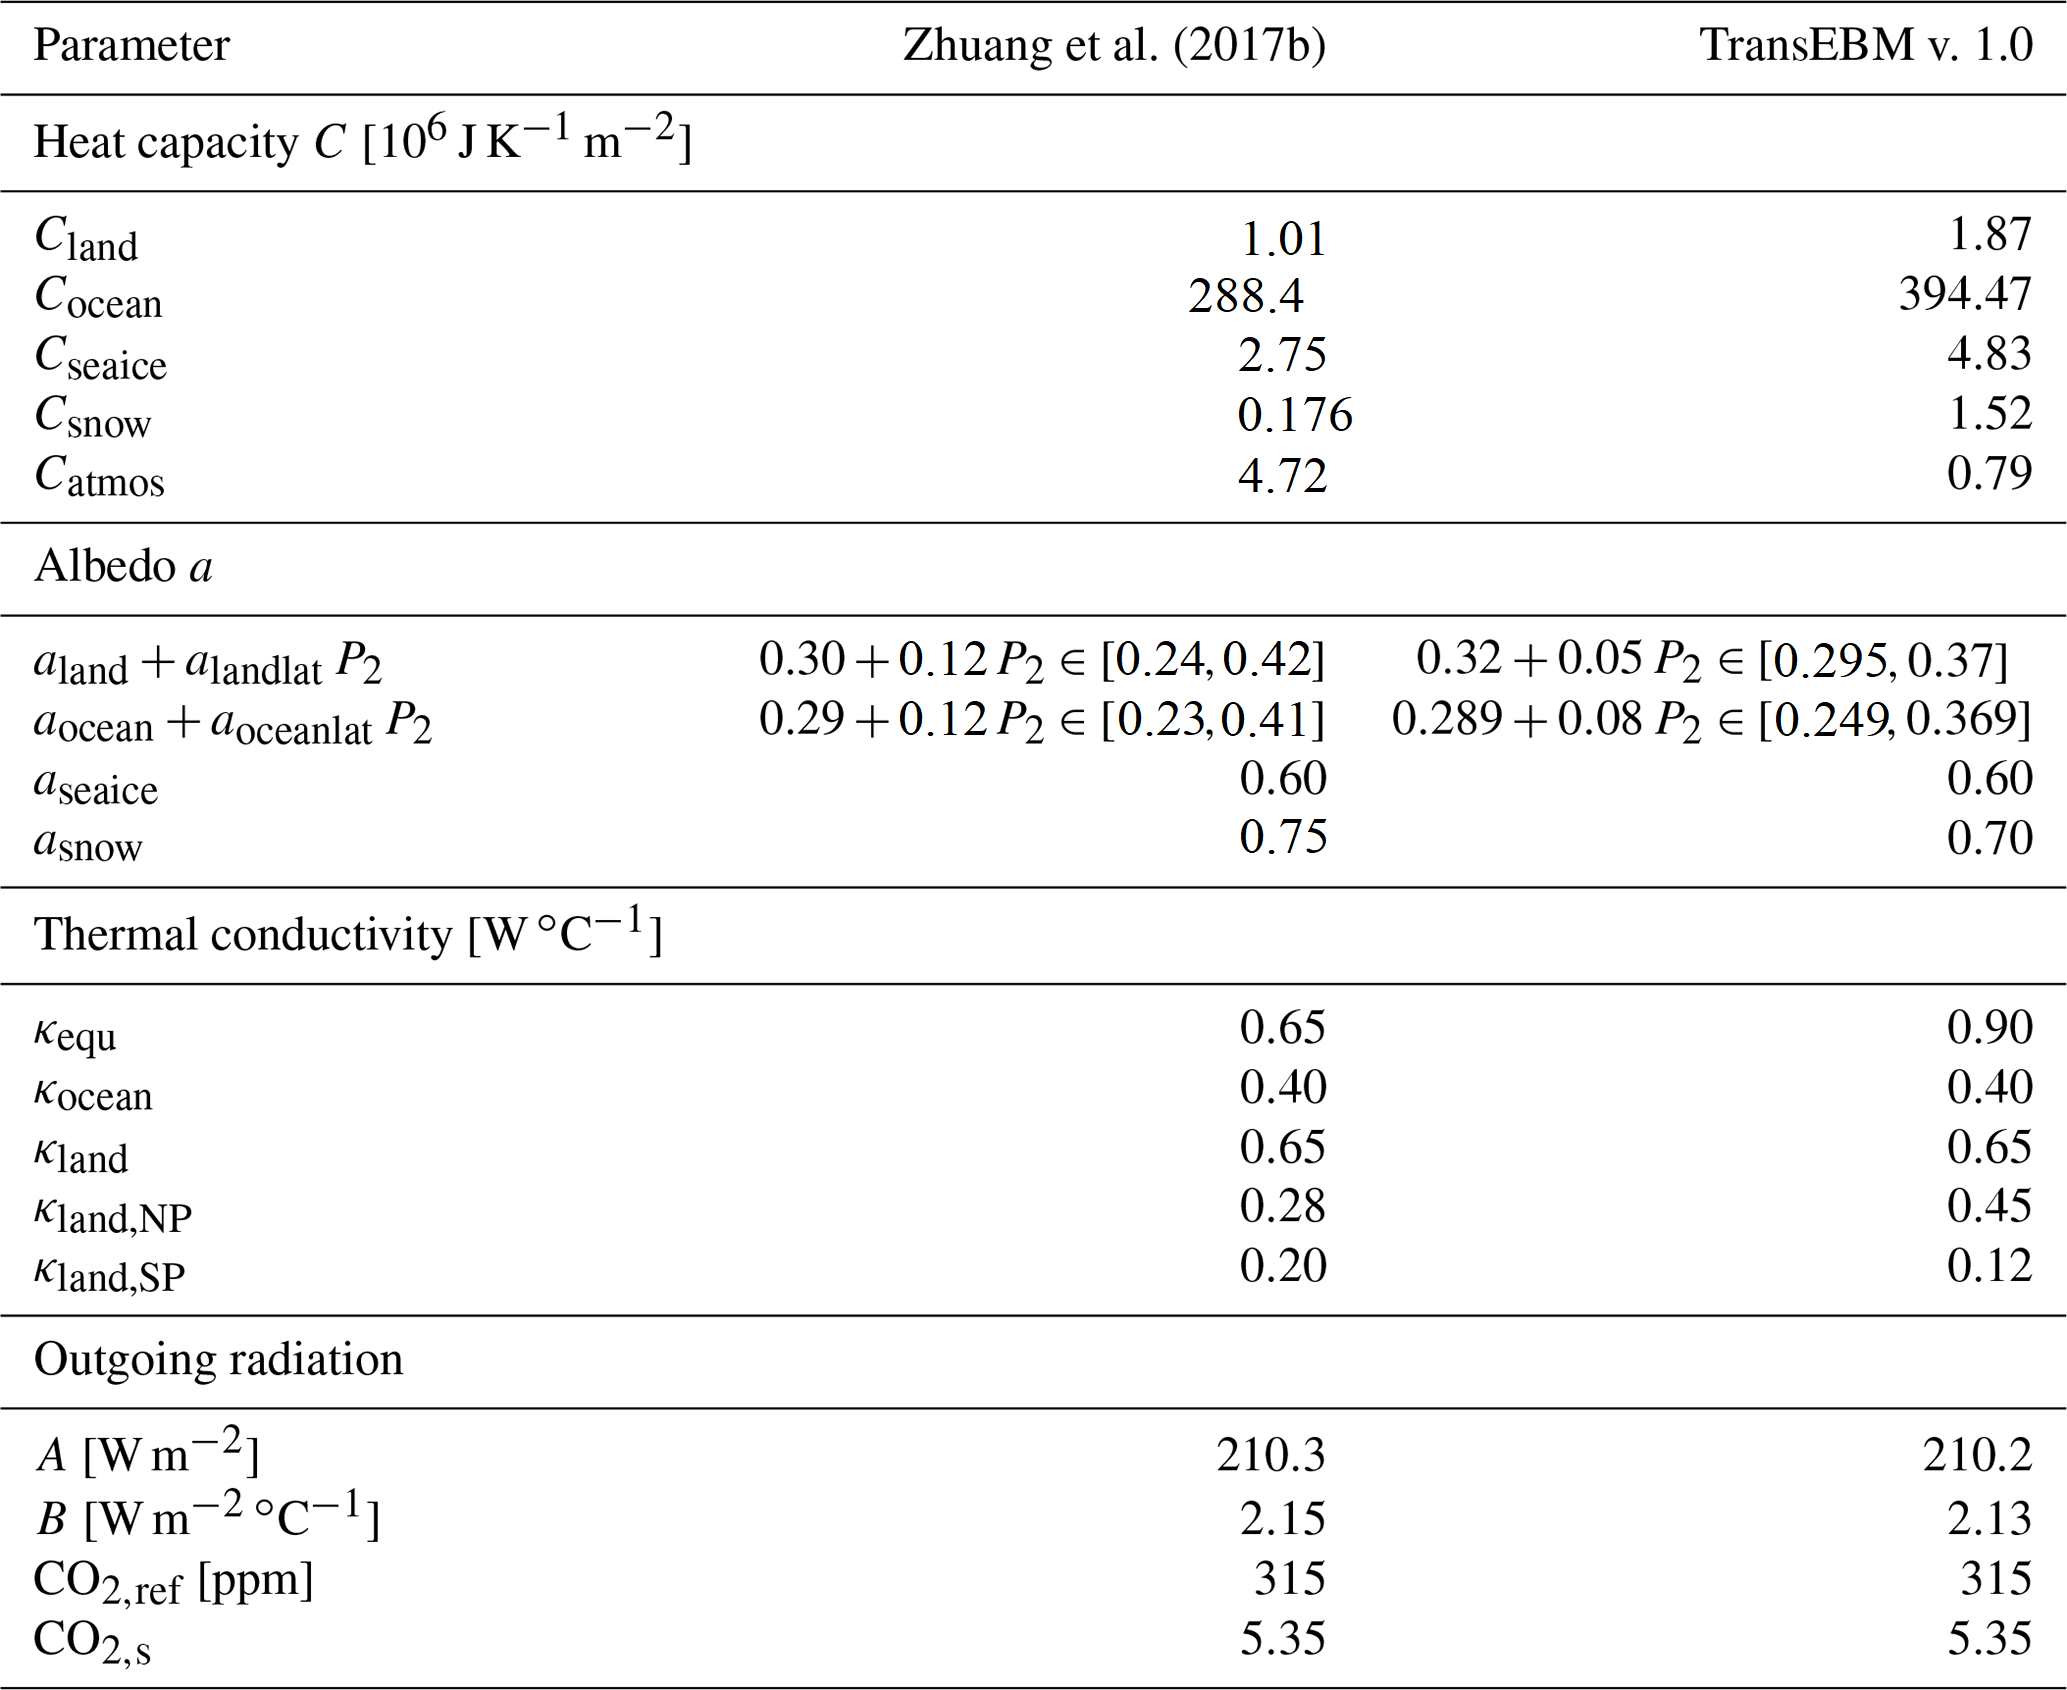
\includegraphics[width=0.7\textwidth,center]{figs/new_parameter.png}
\end{figure}

Note that we have corrected the values for the first column to match the parameters used in this lecture and corrected the intervals for the albedo.\\

Compare your results with the temperatures calculated in 1.

\item Compute the equilibrium temperature from 1980 to present with the NASA $CO_2$ data as in task 3 but with the new parameter. Compare your results.
\end{enumerate}


\section{Control Solutions}

\begin{figure}[!htb]
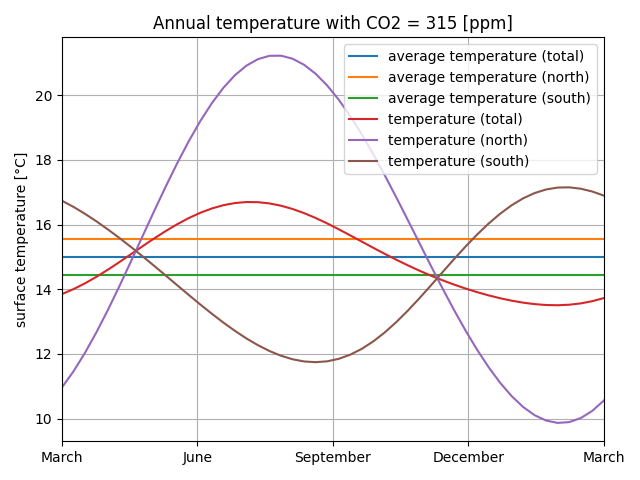
\includegraphics[width=0.6\linewidth,center]{figs/annual_temperature_milestone_6.png}
\caption{2D EBM results for the mean temperatures}
\end{figure}

\begin{figure}[!htb]
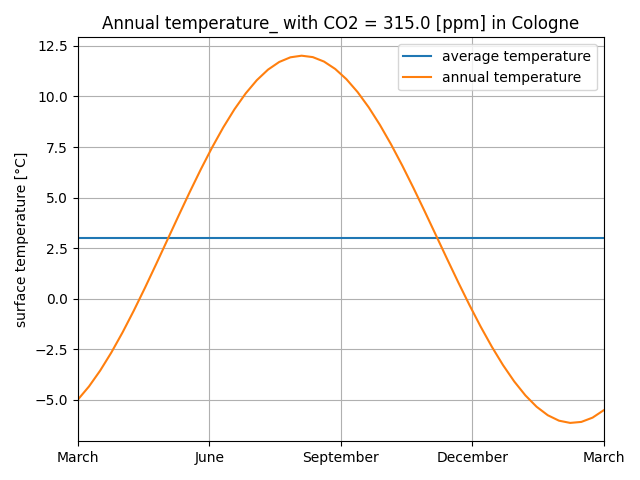
\includegraphics[width=0.6\linewidth,center]{figs/temperature_cologne_milestone_6.png}
\caption{2D EBM results for the temperature in Cologne}
\end{figure}

\begin{figure}[!htb]

\includegraphics[width=0.6\linewidth,center]{figs/annual_temperature_day_80.png}
\caption{2D EBM results for the temperatures on day 80}
\end{figure}

\begin{figure}[!htb]
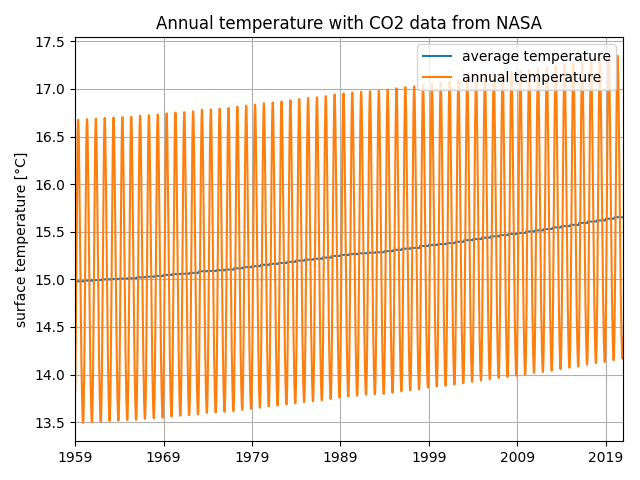
\includegraphics[width=0.7\linewidth,center]{figs/annual_temperatures_nasa.png}
\caption{2D EBM based on NASA data}
\end{figure}



\end{document}
